%%%%%%%%%%%%%%%%%%%%%%%%%%%%%%%
\chapter{CompressibleFlowSolver: Solving the Compressible Navier-Stokes Equations}

In this chapter, we walk the reader through our 2D and 3D compressible Navier-Stokes Solver (CompressibleFlowSolver). 
\section{Fundamental Theories of CompressibleFlowSolver}
\subsection{{Governing equations}}\label{sec:CompNSEqs}
      The governing compressible Navier-Stokes equations, representing conservation of mass, momentum and energy, can be written in abridged form as
      \begin{equation}\label{eq:NS-Eqs}
          \frac{\partial \textbf{U}}{\partial t} = \textit{L}\left(\textbf{U}\right) = -\mathbf{\nabla}\cdot\mathbf{H}\; ; \qquad  \textbf{H}_{i} = 
          \textbf{F}_{i}(\textbf{U}) -
              \textbf{G}_{i}(\textbf{U},\nabla \textbf{U}), 
      \end{equation}
      where $\textit{L}$ is the analytical nonlinear spatial operator, $\textbf{U}$ is the vector of conservative variables, $\textbf{F}=\textbf{F}(\textbf{U})$ is the inviscid flux and $\textbf{G}=\textbf{G}(\textbf{U},\nabla \textbf{U})$ is the viscous flux.
    \subsection{{Discretization}}\label{sec:Spatial-discretization}

    \subsubsection{{Spatial discretization}}
      Various spatial discretization methods are supported, for example the WeakDG and FR for advection term, LDG  and IP methods for the diffusion term. Here, we take the weakDG as example. The computational domain ($\Omega$)
      is divided into $N_{e}$ non-overlapping elements ($\Omega_{e}$).
      The weak form of Eqs. \eqref{eq:NS-Eqs} is obtained by multiplying the test function $\phi_{p}$ and performing integration by parts in $\Omega_{e}$,
      \begin{equation}
          \intop_{\Omega_{e}}\frac{\partial\mathbf{U}}{\partial t}\phi_{p}d\Omega_{e}=\intop_{\Omega_{e}}\mathbf{\nabla}\phi_{p}\cdot\mathbf{H}d\Omega_{e}-\intop_{\varGamma_{e}}\phi_{p}\mathbf{H}^{n}d\varGamma_{e}.\label{eq:weak-integration}
      \end{equation}
      The fluxes are calculated at some quadrature points and a quadrature rule with $N_{Q}$ quadrature points is adopted to calculate the integration in the element and $N_{Q}^{\varGamma}$ quadrature points on element boundaries. This leads to
      \begin{equation}
          \begin{aligned}\sum_{i=1}^{N_{Q}}\sum_{q=1}^{N}\phi_{p}\left(\mathbf{x}_{i}\right)w_{i}J_{i}\phi_{q}\left(\mathbf{x}_{i}\right)\frac{d\mathbf{u}_{q}}{dt}= & \sum_{i=1}^{N_{Q}}w_{i}J_{i}\mathbf{\nabla}\phi_{p}\left(\mathbf{x}_{i}\right)\cdot\mathbf{H}\left(\mathbf{U}_{\delta,i}\right) 
          \\ 
          & -\sum_{i=1}^{N_{Q}^{\varGamma}}\phi_{p}\left(\mathbf{x}_{i}^{\varGamma}\right)w_{i}^{\varGamma}J_{i}^{\varGamma}\hat{\mathbf{H}}_{i}^{n},
          \end{aligned}
          \label{eq:discrete-form-Equations}
      \end{equation}
      where ${\mathbf{u}_{q}}$ is the coefficient vector of the basis function. 
      The whole discretization can
      be written in the following matrix form
      \begin{equation}
          \begin{aligned}
            \frac{d\mathbf{u}}{dt} 
            & = \,\mathbf{M}^{-1} \textit{L}_{\delta}\left(\mathbf{U}\right) = \mathcal{L}_\delta \left(\textbf{u}_{\delta}\right)                          \\
            & = \,\mathbf{M}^{-1}\left[\sum_{j=1}^{d}\mathbf{B}^{T}\mathbf{D}_{j}^{T}\mathbf{\Lambda}\left(wJ\right)\mathbf{H}_{j} -\left(\mathbf{B}^{\varGamma}\mathbf{M_{c}}\right)^{T}\mathbf{\Lambda}\left(w^{\varGamma}J^{\varGamma}\right)\hat{\mathbf{H}}^{n} \right],
          \end{aligned}
          \label{eq:matrix-form-equations}
      \end{equation}
      where $d$ is the spatial dimension,  $\mathbf{M}=\mathbf{B}^{T}\mathbf{\Lambda}\left(wJ\right)\mathbf{B}$
      is the mass matrix, $\mathbf{\Lambda}$ represents
      a diagonal matrix, $\mathbf{D}_{j}$ is the derivative matrix in
      the $j$th direction, $\mathbf{B}^{\varGamma}$ is the backward transformation
      matrix of $\phi^{\varGamma}$ and $\mathbf{M_{c}}$
      is the mapping matrix between $\phi^{\varGamma}$ and $\phi$, $\mathbf{J}$ is the interpolation matrix from quadrature points of a element to quadrature points of its element boundaries.

      The weak DG scheme for the advection term is complete as long as a
      Riemann numerical flux is used to calculate the normal flux,
      $\hat{\mathbf{F}}^{n}\left(\mathbf{Q}^{+},\mathbf{Q}^{-},\mathbf{n}\right)$,
      in which $\mathbf{Q}^{+}$ and $\mathbf{Q}^{-}$ are variable values
      on the exterior and interior sides of the element boundaries, respectively. Similarly, LDG or IP methods are needed to provide the numerical fluxes on element boundaries for the diffusion terms.
    \subsubsection{{Time discretization}}\label{sec:temporalDiscretization}
      Various multi-step and multi-stage methods have been implemented in an object-oriented general linear methods framework. Here, the Runge-Kutta methods are took as examples. The $i$th stage of the Runge-Kutta method is             
          
      \begin{equation}\label{eq:ESDIRKStages_coeffS}
              \textbf{s}^{(i)}
        =\textbf{u}^{n}+\Delta t \sum^{i-1}_{j=1}{a_{ij}\mathcal{L}_\delta\left(\textbf{u}_{\delta}^{(j)}\right)}
        , i=1,2...s    
      \end{equation}
      \begin{equation}\label{eq:ESDIRKStages_coeff}
        \textbf{u}^{(i)}=\textbf{s}^{(i)}+\Delta t a_{ii} \mathcal{L}_\delta\left(\textbf{u}^{(i)}\right)
        , i=1,2...s  
      \end{equation}    
      \begin{equation}
          \textbf{U}_{\delta}^{(i)} = \textbf{B} \textbf{u}^{(i)},\label{eq:ESDIRKStages_coeffBWD}
      \end{equation}
      where $a_{ij}$ is the coefficient of the Runge-Kutta method, $\textbf{s}$ is a source term, $\textbf{B}$ is  the backward transform matrix.
      Finally, the solution of the new time step ($n+1$) is calculated by
      \begin{equation}\label{eq:URKUpdate}
        \textbf{U}^{n+1}=\textbf{U}^{n}+\Delta t\sum^{s}_{i=1}{b_{i} \textit{L}\left(\textbf{U}^{(i)}\right)}
        ,
      \end{equation}
      For explicit RK methods, $a_{ii} =0$, the discretization is complete and straightforward. 
    \subsubsection{{Jacobian-free Newton-Krylov method}}\label{sec:Newton-Krylov}
      
      Eq.~\eqref{eq:ESDIRKStages_coeff} of the implicit stages ($a_{ii} \neq 0$) can be written as the nonlinear system  
      \begin{equation}\label{eq:NonlinSys}
          \textbf{N}(\textbf{u}_{\delta}^{(i)})=\textbf{u}_{\delta}^{(i)} - \textbf{s}^{(i)}-\Delta t a_{ii} \mathcal{L}_\delta\left(\textbf{u}_{\delta}^{(i)}\right) = \textbf{0}.
      \end{equation}
      This system is iteratively solved by Newton's method \cite{knoll_jacobian_free_2004} with the Newton step, $\Delta \textbf{v}=\textbf{v}^{k+1}-\textbf{v}^{k}$, updated through the solution of the linear system 
      \begin{equation}\label{eq:NewtonIte}
          \frac{\partial \textbf{N}(\textbf{v}^{k})}{\partial \textbf{v}}\Delta \textbf{v}=-\textbf{N}(\textbf{v}^{k}).
      \end{equation}
      where $\textbf{v}^{0} = \textbf{s}^{(i)}$ is adopted as an initial guess. When the Newton residual is smaller than the convergence tolerance  of the Newton iterations $\tau$, which is 
      \begin{equation}\label{eq:NewtonTol}
      \lVert \textbf{N}(\textbf{v}^{k}) \rVert = \lVert \textbf{R}(\textbf{v}^{k}) \rVert \leq \tau,
      \end{equation}
      $\textbf{u}_{it}^{(i)} = \textbf{v}^{k}$ is regarded as the approximate solution of the nonlinear system, where $\textbf{R}$ is the remaining Newton residual vector $\textbf{N}(\textbf{u}^{(i)}_{it})$ after convergence. 
      
      The restarted generalized minimal residual method (GMRES) \cite{saad_gmres:_1986} is used for solving the linear problem \eqref{eq:NewtonIte}. The Jacobian matrix and vector inner product operator is approximated by the following finite difference 
      \begin{equation}
          \frac{\partial\mathbf{N}}{\partial\mathbf{u}}\left(\mathbf{u}\right)\cdot\mathbf{q} \simeq \frac{\mathbf{N}(\mathbf{u}+\epsilon\mathbf{q})-\mathbf{N}(\mathbf{u})}{\epsilon},\label{eq:Jacobian-free-matrix}
      \end{equation}
      where $\epsilon$ is the step size of the finite difference approximation.

      The use of good preconditioners in GMRES is very important for efficiently solving stiff linear systems. Instead of solving the system of Eq. \eqref{eq:NewtonIte} directly, one can get the same solution by solving the preconditioned linear system
      \begin{equation}
          \left(\frac{\partial\mathbf{N}}{\partial\mathbf{u}}\mathbf{P}^{-1}\right)\left(\mathbf{P}\bigtriangleup\bar{\mathbf{u}}^{l}\right)=-\mathbf{N}\left(\bar{\mathbf{u}}^{l}\right),\label{eq:preconditioning}
      \end{equation}
      where $\mathbf{P}$ is the preconditioning matrix. A low memory block relaxed Jacobi iterative preconditioner is implemented.


  \section{Functions of the implementation}
    
    Table \ref{tab:CFSFunctionName} lists the 
    main functions of the explicit and implicit compressible flow solver. 
    The discretization of the advection term mainly uses the \texttt{ AdvectVolumeFlux} and 
    \texttt{ AdvectTraceFlux} to calculate the fluxes on the quadrature points of inside the element and on the element boundaries. 
    Then, \texttt{ IProductWRTDerivBase} and \texttt{ AddTraceIntegral} are adopted to perform the integrations. 
    Similarly, in the diffusion discretization, \texttt{ DiffuseVolumeFlux} and \texttt{ DiffuseTraceFlux} are implemented for calculating the fluxes, while \texttt{ IProductWRTDerivBase} and \texttt{ AddTraceIntegral} are for the integrations. For the diffusion term, spatial derivatives are needed and calculated using \texttt{ DiffuseCalcDerivative}. For the interior penalty method an extra symmetric term may be needed and calculated by \texttt{ AddDiffusionSymmFluxToCoeff}. The above functions forms the spatial operator of \texttt{ DoOdeRhs} and the explicit solver in relatively complete coupled with a explicit time integration scheme. For the implicit solver, extra functions are needed. The \texttt{ DoImplicitSolve} solves the nonlinear system, in which the \texttt{ NonlinSysEvaluatorCoeff1D} evaluates the nonlinear system residual, \texttt{ MatrixMultiplyMatrixFreeCoeff} calculates the Jacobian matrix vector inner product and \texttt{ PreconCoeff} perform the preconditioning. Provided a specific implicit time integration scheme, the \texttt{ DoImplicitSolve} helps solve the nonlinear system for implicit stages and the implicit solver is complete.
   
    \begin {table}[htbp!]
    \caption {Table of variable and function mapping used in the compressible flow solver to their mathematical operations} \label{tab:CFSFunctionName} 
    \begin{center}
    \scalebox{0.9}[1.]{
    \begin{tabular}{ | l | l|}
      \hline      
      \textbf{ Variable/Function name} & \textbf{ Physical meaning} \\  
      \hline
      \texttt{ AdvectVolumeFlux}  & Advection Euler flux: $\textbf{F}_{i}$\\
      \hline
      \texttt{ AdvectTraceFlux}  & Advection (Riemann) numerical flux at trace: $\hat{\textbf{F}}_{i}$\\
      \hline
      \texttt{ IProductWRTDerivBase} &  $\sum_{j=1}^{d}\mathbf{B}^{T}\mathbf{D}_{j}^{T}\mathbf{\Lambda}\left(wJ\right)$ operator to a vector\\
      \hline
      \texttt{ AddTraceIntegral} &  $\left(\mathbf{B}^{\varGamma}\mathbf{M_{c}}\right)^{T}\mathbf{\Lambda}\left(w^{\varGamma}J^{\varGamma}\right)$ to a vector\\ 
      \hline
      \texttt{ MultiplyByElmImvMass} & Multiply the inverse of mass matrix to a vector\\
      \hline
      \texttt{ DiffuseCalcDerivative} & Calculate the derivatives of a vector\\
      \hline
      \texttt{ DiffuseVolumeFlux} & Analytical Diffusion flux: $\textbf{G}_{i}$ \\
      \hline
      \texttt{ DiffuseTraceFlux} & Calculate the diffusion numerical flux $ \hat{\textbf{G}}$\\
      \hline
      \texttt{ AddDiffusionSymmFluxToCoeff} & Add the integral of symmetric flux (special for IP)\\
      \hline
      \texttt{ DoOdeRhs} & Calculate $\mathcal{L}_\delta \left(\textbf{u}_{\delta}\right)$\\
      \hline
      \texttt{ DoImplicitSolve} & Solve the nonlinear system in implicit time integrations\\
      \hline
      \texttt{ NonlinSysEvaluatorCoeff1D} & Calculate $\textbf{N}(\textbf{u}_{\delta}^{(i)})$\\
      \hline
      \texttt{ MatrixMultiplyMatrixFreeCoeff} & Calculate ${\partial\mathbf{N}}/{\partial\mathbf{u}}\left(\mathbf{u}\right)\cdot\mathbf{q}$\\
      \hline
      \texttt{ PreconCoeff} & Perform preconditioning\\
      \hline
    \end{tabular}
    }
    \end{center}
    \end{table}

\section{Data Structure of CompressibleFlowSolver}
   \begin{figure}
          \caption{CompressibleFlowSolver DataStructure}
        \centering
        \begin{turn}{90}
        \includestandalone[width=1.2\linewidth]{DataStructure}
        \end{turn}
    \end{figure}

\clearpage
\section{Flow Chart of CompressibleFlowSolver}
    
  \begin{figure}[htbp!]
    \begin{centering}
        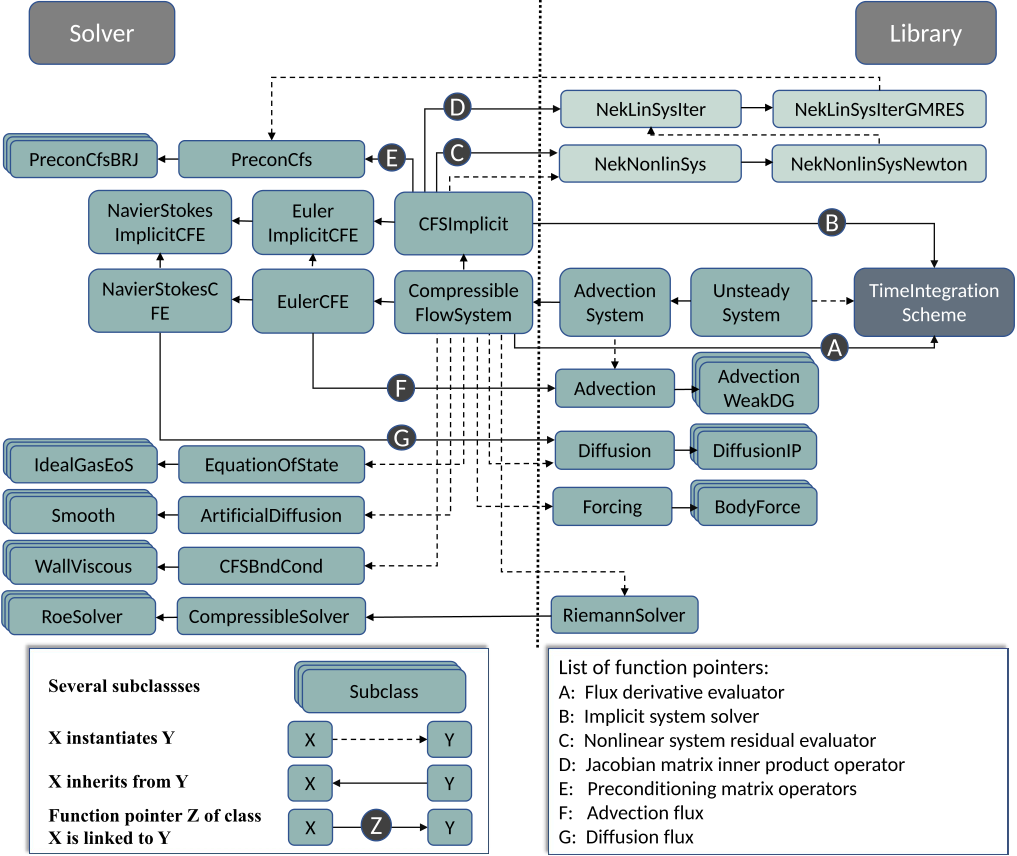
\includegraphics[width=1\textwidth]{./img/DataStructureFinal}
        \par\end{centering}
    \centering{}\caption{Class structure of the explicit and implicit solvers. The equation system classes ($\texttt{ EulerCFE}$ or $\texttt{ NavierStokesCFE}$) contain access to the main functionalities of the solver, such as time integration, and the solution fields. They make use of numerical methods from the libraries, such as $\texttt{ AdvectionWeakDG}$, and equations system related functions, such as the advection flux ($\texttt{ F}$) and diffusion flux ($\texttt{ G}$), to form the spatial discretization operator $\texttt{ A}$. The spatial operator $\texttt{ A}$ and the time integration method form the explicit solver using the method of lines. For the implicit solver, additional classes like the Newton solver ($\texttt{ NekNonlinSysNewton}$), GMRES solver ($\texttt{ NekLinSysIterGMRES}$) and linear algebra solver of preconditioners (e.g. $\texttt{ PrecondCfsBRJ}$) are instantiated. Together with operators related to the nonlinear system ($\texttt{ C}$), the Jacobian matrix ($\texttt{ D}$) and preconditioning matrix ($\texttt{ E}$), an implicit system solver ($\texttt{ B}$) is constructed, which is linked to the implicit time integration scheme to form the implicit solver.} \label{fig:Class-structure-of}
  \end{figure}
  

  The main procedures for building a solver are briefly introduced using
  the explicit solver of the NS equations as an example. Besides the main
  solver class ($\texttt{ CompressibleFlowSolver}$) which controls the
  solving procedure, an equation system class is needed. The
  equation system classes ($\texttt{ EulerCFE}$ or $\texttt{ NavierStokesCFE}$)
  are instantiated and initialized dynamically based on user inputs using
  a factory method pattern \cite{Cantwell2015}, which is also extensively
  used for the dynamic object creation of classes in the solver. The equation
  system class inherits instantiations of classes related to geometry
  information, solution approximation, time integration and others from
  equations system classes in the libraries such as $\texttt{ UnsteadySystem}$
  in $\texttt{ SolverUtils}$. Thus the main functionality of the equation system class
  is to offer equation system related functions and to form spatial
  discretization operators using numerical methods from the libraries
  such as, $\texttt{ AdvectionWeakDG}$. Fig.~\ref{fig:Class-structure-of}
  illustrates the class structure of the explicit and implicit solvers.
  The equation of state ($\texttt{ EquationOfState}$), boundary conditions
  ($\texttt{ CFSBndCond}$), Riemann flux ($\texttt{ RiemmanSolver}$), shock
  capturing method ($\texttt{ ArtificialDiffusion}$), forcing term ($\texttt{ Forcing}$),
  advection flux (function pointer $\texttt{ F}$) and diffusion flux (function
  pointer $\texttt{ G}$) are instantiated or implemented in the equation system class.
  Specific numerical schemes like the weak
  DG scheme for advection terms ($\texttt{ AdvectionWeakDG}$) and the interior
  penalty method for diffusion terms ($\texttt{ DiffusionIP}$) are instantiated
  to calculate $\mathbf{\nabla}\cdot\mathbf{F}$
  and $\mathbf{\nabla}\cdot\mathbf{G}$ in Eq. \eqref{eq:NS-Eqs}
  provided with all these equation system related functions ($\texttt{ F}$ and $\texttt{ G}$). Finally
  the spatial discretization operator $\textit{L}_{\delta}\left(\mathbf{u},t\right)$
  is linked to the time integration class using the pointer-to-function
  $\texttt{ A}$ and the explicit solver is complete.

  The main simulation flowchart of the implicit solver is given in Tab. \ref{tab:Cfs-NSFlow-chart}, which also shows the flow between different classes.
  \begin {table}[htbp!]
    \caption {Nassi--Shneiderman diagram of the implicit solver with the corresponding
    class names. Brown: library class ; cyan: solver class.} \label{tab:Cfs-NSFlow-chart} 
  \begin{tabular}{|l|l|l|l|l|l||ll||l||l||l||l||l|}
    \hline 
    \multicolumn{7}{|l}{Initialization} & \multicolumn{6}{l|}{{\footnotesize{}in }\textcolor{cyan}{\footnotesize{}$\texttt{CompressibleFlowSolver}$}}\tabularnewline
    \hline 
    \multicolumn{7}{|l}{Time step loop $n$} & \multicolumn{6}{l|}{{\footnotesize{}in }\textcolor{brown}{\footnotesize{}$\texttt{UnsteadySystem}$}}\tabularnewline
    \cline{2-13} \cline{3-13} \cline{4-13} \cline{5-13} \cline{6-13} \cline{7-13} \cline{8-13} \cline{9-13} \cline{10-13} \cline{11-13} \cline{12-13} \cline{13-13} 
    \multirow{12}{*}{} & \multicolumn{6}{l}{Runge-Kutta loop $m=1,\cdots,M$} & \multicolumn{6}{l|}{{\footnotesize{}in }\textcolor{brown}{\footnotesize{}$\texttt{TimeIntegrationScheme}$}}\tabularnewline
    \cline{3-13} \cline{4-13} \cline{5-13} \cline{6-13} \cline{7-13} \cline{8-13} \cline{9-13} \cline{10-13} \cline{11-13} \cline{12-13} \cline{13-13} 
     & \multirow{10}{*}{} & \multicolumn{5}{l}{Calculate source term $\mathbf{S}_{m}$} & \multicolumn{6}{l|}{{\footnotesize{}in }\textcolor{brown}{\footnotesize{}$\texttt{TimeIntegrationScheme}$}}\tabularnewline
    \cline{3-13} \cline{4-13} \cline{5-13} \cline{6-13} \cline{7-13} \cline{8-13} \cline{9-13} \cline{10-13} \cline{11-13} \cline{12-13} \cline{13-13} 
     &  & \multicolumn{5}{l}{Netwon iteration $l$} & \multicolumn{6}{l|}{{\footnotesize{}in }\textcolor{brown}{\footnotesize{}$\texttt{NewtonSolver}$}}\tabularnewline
    \cline{4-13} \cline{5-13} \cline{6-13} \cline{7-13} \cline{8-13} \cline{9-13} \cline{10-13} \cline{11-13} \cline{12-13} \cline{13-13} 
     &  & \multirow{8}{*}{} & \multicolumn{4}{l}{Calculate residual $\mathbf{N}\left(\bar{\mathbf{u}}^{l}\right)$} & \multicolumn{6}{l|}{{\footnotesize{}in }\textcolor{cyan}{\footnotesize{}$\texttt{CFSImplicit}$}}\tabularnewline
    \cline{4-13} \cline{5-13} \cline{6-13} \cline{7-13} \cline{8-13} \cline{9-13} \cline{10-13} \cline{11-13} \cline{12-13} \cline{13-13} 
     &  &  & \multicolumn{4}{l}{GMRES iteration $k$} & \multicolumn{6}{l|}{{\footnotesize{}in }\textcolor{brown}{\footnotesize{}$\texttt{NekLinSysIterGMRES}$}}\tabularnewline
    \cline{5-13} \cline{6-13} \cline{7-13} \cline{8-13} \cline{9-13} \cline{10-13} \cline{11-13} \cline{12-13} \cline{13-13} 
     &  &  & \multirow{5}{*}{} & \multicolumn{3}{l}{Calculate search vector $\mathbf{q}_{k}$} & \multicolumn{6}{l|}{{\footnotesize{}in }\textcolor{brown}{\footnotesize{}$\texttt{NekLinSysIterGMRES}$}}\tabularnewline
    \cline{5-13} \cline{6-13} \cline{7-13} \cline{8-13} \cline{9-13} \cline{10-13} \cline{11-13} \cline{12-13} \cline{13-13} 
     &  &  &  & \multicolumn{3}{l}{BRJ iteration $j=1,\cdots,J$ } & \multicolumn{6}{l|}{{\footnotesize{}in }\textcolor{brown}{\footnotesize{}$\texttt{PrecondBRJ}$}}\tabularnewline
    \cline{6-13} \cline{7-13} \cline{8-13} \cline{9-13} \cline{10-13} \cline{11-13} \cline{12-13} \cline{13-13} 
     &  &  &  &  & \multicolumn{2}{l}{Calculate {\small{}$\hat{\mathbf{q}}^{j}=\hat{\mathbf{D}}^{-1}\left(\mathbf{q}_{k}-\left(\mathbf{\hat{L}}+\hat{\mathbf{U}}\right)\hat{\mathbf{q}}^{j-1}\right)$}} & \multicolumn{6}{l|}{{\footnotesize{}in }\textcolor{cyan}{\footnotesize{}$\texttt{CFSImplicit}$}}\tabularnewline
    \cline{5-13} \cline{6-13} \cline{7-13} \cline{8-13} \cline{9-13} \cline{10-13} \cline{11-13} \cline{12-13} \cline{13-13} 
     &  &  &  & \multicolumn{3}{l}{Calculate $\partial\mathbf{N}/\partial\mathbf{u}\cdot\hat{\mathbf{q}}^{J}$} & \multicolumn{6}{l|}{{\footnotesize{}in }\textcolor{cyan}{\footnotesize{}$\texttt{CFSImplicit}$}}\tabularnewline
    \cline{5-13} \cline{6-13} \cline{7-13} \cline{8-13} \cline{9-13} \cline{10-13} \cline{11-13} \cline{12-13} \cline{13-13} 
     &  &  &  & \multicolumn{3}{l}{Calculate linear system residual} & \multicolumn{6}{l|}{{\footnotesize{}in }\textcolor{brown}{\footnotesize{}$\texttt{NekLinSysIterGMRES}$}}\tabularnewline
    \cline{4-13} \cline{5-13} \cline{6-13} \cline{7-13} \cline{8-13} \cline{9-13} \cline{10-13} \cline{11-13} \cline{12-13} \cline{13-13} 
     &  &  & \multicolumn{4}{l}{Calculate $\bar{\mathbf{u}}^{l+1}$ by linear combination of $\mathbf{q}_{k}$} & \multicolumn{6}{l|}{{\footnotesize{}in }\textcolor{brown}{\footnotesize{}$\texttt{NekLinSysIterGMRES}$}}\tabularnewline
    \cline{2-13} \cline{3-13} \cline{4-13} \cline{5-13} \cline{6-13} \cline{7-13} \cline{8-13} \cline{9-13} \cline{10-13} \cline{11-13} \cline{12-13} \cline{13-13} 
     & \multicolumn{6}{l}{Calculate $\mathbf{u}^{n+1}$} & \multicolumn{6}{l|}{{\footnotesize{}in }\textcolor{brown}{\footnotesize{}$\texttt{TimeIntegrationScheme}$}}\tabularnewline
    \hline 
    \multicolumn{7}{|l}{Output and finalization} & \multicolumn{6}{l|}{{\footnotesize{}in }\textcolor{cyan}{\footnotesize{}$\texttt{CompressibleFlowSolver}$}}\tabularnewline
    \hline 
    \end{tabular}
  \end{table}

   %% \begin{figure}
   %%        \caption{CompressibleFlowSolver Main Flow Chart}
   %%      \centering
   %%    \begin{tikzpicture}[scale=0.2,node distance=1cm]
   %%    \node (A)
   %%    [rectangle,
   %%    rounded corners,
   %%    minimum width=8cm,
   %%    minimum height=1cm,
   %%    text centered,
   %%    draw=black,
   %%    fill=red!30]
   %%    {CompressibleFlowSolver$.$cpp};
   %%    \node (B_1)
   %%    [rectangle,
   %%    rounded corners,
   %%    minimum width=8cm,
   %%    minimum height=1cm,
   %%    text width=8cm,
   %%    text centered,
   %%    draw=black,
   %%    fill=blue!20,
   %%    below =of A,
   %%    xshift=0cm,
   %%    yshift=0cm]
   %%    {Initialize Objects\\eg. DriverStandard::v$\_$InitObject\\See Figure \ref{fig1}};
   %%    \draw[arrow](A)--(B_1);
   %%    \node (B_2)
   %%    [rectangle,
   %%    rounded corners,
   %%    minimum width=8cm,
   %%    minimum height=1cm,
   %%    text width=8cm,
   %%    text centered,
   %%    draw=black,
   %%    fill=blue!20,
   %%    below =of B_1,
   %%    xshift=0cm,
   %%    yshift=0cm]
   %%    {Execute Solver beginning from driver:\\eg. DriverStandard::v$\_$Execute};
   %%    \draw[arrow](B_1)--(B_2);
   %%    \node (C_1)
   %%    [rectangle,
   %%    rounded corners,
   %%    minimum width=8cm,
   %%    minimum height=1cm,
   %%    text width=8cm,
   %%    text centered,
   %%    draw=black,
   %%    fill=yellow!20,
   %%    right= of B_2,
   %%    xshift=0cm,
   %%    yshift=0cm]
   %%    {Initial conditions: \\m$\_$equ[0]-$>$DoInitialise\\ See Figure \ref{fig2}};
   %%    \draw[arrow](B_2.east)--(C_1);
   %%    \node (C_2)
   %%    [rectangle,
   %%    rounded corners,
   %%    minimum width=8cm,
   %%    minimum height=1cm,
   %%    text width=8cm,
   %%    text centered,
   %%    draw=black,
   %%    fill=yellow!20,
   %%    below = of C_1,
   %%    xshift=0cm,
   %%    yshift=0cm]
   %%    {Main execution of solver:\\m$\_$equ[0]-$>$DoSolve\\ See Figure \ref{fig3} and Figure \ref{fig4}};
   %%    \draw[arrow](B_2.east)--($(B_2.east)+(2cm,0)$)|-(C_2);
   %%    \node (C_3)
   %%    [rectangle,
   %%    rounded corners,
   %%    minimum width=8cm,
   %%    minimum height=1cm,
   %%    text width=8cm,
   %%    text centered,
   %%    draw=black,
   %%    fill=yellow!20,
   %%    below = of C_2,
   %%    xshift=0cm,
   %%    yshift=0cm]
   %%    {Output brief information:\\m$\_$equ[0]-$>$Output};
   %%    \draw[arrow](B_2.east)--($(B_2.east)+(2cm,0)$)|-(C_3);
   %%    \end{tikzpicture}
   %%  \end{figure}
    

%% \clearpage
%%    \begin{figure}
%%           \caption{CompressibleFlowSolver InitObject}\label{fig1}
%%         \centering
%%         \includestandalone[width=1\linewidth]{FlowChart1}
%%     \end{figure}

%% \clearpage
%%    \begin{figure}
%%           \caption{CompressibleFlowSolver Initialize Conditions}\label{fig2}
%%         \centering
%%         \includestandalone[width=1\linewidth]{FlowChart2}
%%     \end{figure}

%% \clearpage
%%    \begin{figure}
%%           \caption{CompressibleFlowSolver Execute Advection}\label{fig3}
%%         \centering
%%         \includestandalone[width=0.5\linewidth]{FlowChart3}
%%    \end{figure}

%% \clearpage
%%    \begin{figure}
%%           \caption{CompressibleFlowSolver Execute Diffusion}\label{fig4}
%%         \centering
%%         \includestandalone[width=0.5\linewidth]{FlowChart4}
%%    \end{figure}


% \section{The Fundamentals Behind the Compressible Flow Solver}

% \subsection{Strong Form of the System}

% \subsection{Variational Form of the System}

% \section{The Fundamentals Behind the Data Structures}

% \subsection{Overview}

% \subsection{Equation System Description}

% \subsection{Advection Components}

% \subsection{Diffusion Components}


% \section{The Fundamental Flow Control of The Solver: Flow Chart}

% \subsection{Top-Down Perspective}

% \subsection{Evaluation of the Explicit Term}

% \subsection{Evaluation of the Implicit Term}

% \section{The Fundamental Algorithms}

% \paragraph{How Would I Change From External Energy Form to Internal Energy Form?}

% \paragraph{How Is De-Aliasing Applied to the Non-Linear Terms?}

